\section{Designing a custom integrator plugin}
Suppose you want to design a custom integrator to render scenes in Mitsuba.
There are two general ways you can do this, and which one you should take
mostly depends on the characteristics of your particular integrator.

The framework distinguishes between \emph{sampling-based} integrators and
\emph{generic} ones. A sampling-based integrator is able to generate
(usually unbiased) estimates of the incident radiance along a specified rays, and this
is done a large number of times to render a scene. A generic integrator
is more like a black box, where no assumptions are made on how the the image is
created. For instance, the VPL renderer uses OpenGL to rasterize the scene
using hardware acceleration, which certainly doesn't fit into the sampling-based pattern.
For that reason, it must be implemented as a generic integrator.

Generally, if you can package up your code to fit into the
\code{SamplingIntegrator} interface, you should do it, because you'll get
parallelization and network rendering essentially for free. This is done
by transparently sending instances of your integrator class to all participating cores
and assigning small image blocks for each one to work on. Also, sampling-based
integrators can be nested within some other integrators, such as an
irradiance cache or an adaptive integrator. This cannot be done with generic
integrators due to their black-box nature. Note that it is often still
possible to parallelize generic integrators, but this involves significantly
more work.

In this section, we'll design a rather contrived sampling-based integrator,
which renders a monochromatic image of your scene, where the intensity
denotes the distance to the camera. But to get a feel for the overall
framework, we'll start with an even simpler one, that just renders a
solid-color image.

\subsection{Basic implementation}
In Mitsuba's \code{src/integrators} directory, create a file named
\code{myIntegrator.cpp}.

\begin{cpp}
#include <mitsuba/render/scene.h>

MTS_NAMESPACE_BEGIN

class MyIntegrator : public SamplingIntegrator {
public:
	MTS_DECLARE_CLASS()
};

MTS_IMPLEMENT_CLASS_S(MyIntegrator, false, SamplingIntegrator)
MTS_EXPORT_PLUGIN(MyIntegrator, "A contrived integrator");
MTS_NAMESPACE_END
\end{cpp}
The \code{scene.h} header file contains all of the dependencies we'll need
for now.
To avoid conflicts with other libraries, the whole framework is located in
a separate namespace named \code{mitsuba}, and the lines starting with
\code{MTS\_NAMESPACE} ensure that our integrator is placed there
as well.

The two lines starting with \code{MTS\_DECLARE\_CLASS} and \code{MTS\_IMPLEMENT\_CLASS}
ensure that this class is recognized as a native Mitsuba class.
This is necessary to get things like run-time type information, reference counting,
and serialization/unserialization support. Let's take a look at the second of these
lines, because it contains several important pieces of information:

The suffix \code{S} in \code{MTS\_IMPLEMENT\_CLASS\_S} specifies that this is
a serializable class, which means that it can be sent over the network or
written to disk and later restored. That also implies that certain methods
need to be provided by the implementation --- we'll add those in a moment.

The three following parameters specify the name of this class (\code{MyIntegrator}),
the fact that it is \emph{not} an abstract class (\code{false}), and the name of its
parent class (\code{SamplingIntegrator}).

Just below, you can see a line that starts with
\code{MTS\_EXPORT\_PLUGIN}. As the name suggests, this line is only necessary
for plugins, and it ensures that the specified class (\code{MyIntegrator}) is
what you want to be instantiated when somebody loads this plugin. It is also
possible to supply a short descriptive string.
\vspace{3mm}

Let's add an instance variable and a constructor:
\begin{cpp}
public:
    /// Initialize the integrator with the specified properties
    MyIntegrator(const Properties &props) : SamplingIntegrator(props) {
        Spectrum defaultColor;
        defaultColor.fromLinearRGB(0.2f, 0.5f, 0.2f);
        m_color = props.getSpectrum("color", defaultColor);
    }

private:
	Spectrum m_color;
\end{cpp}

This code fragment sets up a default color (a light shade of green), which
can be overridden from the scene file. For example, one could instantiate
the integrator from an XML document like this

\begin{xml}
<integrator type="myIntegrator">
	<spectrum name="color" value="1.0"/>
</integrator>
\end{xml}
in which case white would take preference.
\vspace{3mm}

Next, we need to add serialization and unserialization support:
\begin{cpp}
    /// Unserialize from a binary data stream
    MyIntegrator(Stream *stream, InstanceManager *manager)
     : SamplingIntegrator(stream, manager) {
        m_color = Spectrum(stream);
    }

    /// Serialize to a binary data stream
    void serialize(Stream *stream, InstanceManager *manager) const {
        SamplingIntegrator::serialize(stream, manager);
        m_color.serialize(stream);
    }
\end{cpp}
This makes use of a \emph{stream} abstraction similar in style to Java.
A stream can represent various things, such as a file, a console session, or a
network communication link. Especially when dealing with multiple machines,
it is important to realize that the machines may use different binary representations
related to their respective \emph{endianness}. To prevent issues from arising,
the \code{Stream} interface provides many methods for writing and reading
small chunks of data (e.g. \code{writeShort}, \code{readFloat}, ..),
which automatically perform endianness translation. In our case, the
\code{Spectrum} class already provides serialization/unserialization support,
so we don't really have to do anything.

Note that it is crucial that your code calls the serialization and unserialization
implementations of the superclass, since it will also read/write some
information to the stream.

We haven't used the \texttt{manager} parameter yet, so here is a quick overview
of what it does: if many cases, we don't just want to serialize a single class,
but a whole graph of objects. Some may be referenced many
times from different places, and potentially there are even cycles. If we just
naively called the serialization and unserialization implementation of members
recursively within each class, we'd waste much bandwitdth and potentially
end up stuck in an infinite recursion.

This is where the instance manager comes in. Every time you want to serialize
a heap-allocated object (suppose it is of type \code{SomeClass}),
instead of calling its serialize method, write

\begin{cpp}
ref<SomeClass> myObject = ...;
manager->serialize(stream, myObject.get());
\end{cpp}

Later, to unserialize the object from a stream again, write
\begin{cpp}
ref<SomeClass> myObject = static_cast<SomeClass *>(manager->getInstance(stream));
\end{cpp}

Behind the scenes, the object manager adds annotations to the data stream,
which ensure that you will end up with the exact same reference graph on the
remote side, while only one copy of every object is transmitted and no
infinite recursion can occur. But we digress -- let's go back to our integrator.
\vspace{3mm}

The last thing to add is a function, which returns an estimate for the
radiance along a ray differential: here, we simply return the stored color
\begin{cpp}
    /// Query for an unbiased estimate of the radiance along <tt>r</tt>
   Spectrum Li(const RayDifferential &r, RadianceQueryRecord &rRec) const {
       return m_color;
   }
\end{cpp}

Let's try building the plugin: edit the \code{SConstruct} file in the main
directory, and add the following line after the comment ''\code{\# Integrators}'':
\begin{cpp}
plugins += env.SharedLibrary('plugins/myIntegrator', ['src/integrators/myIntegrator.cpp'])
\end{cpp}
After calling, \texttt{scons}, you should be able to use your new integrator
in parallel rendering jobs and you'll get something like this:
\begin{center}
\scalebox{.4}{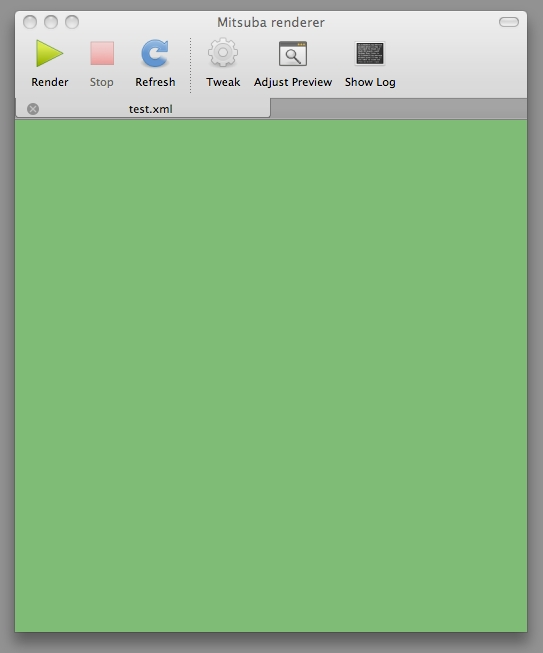
\includegraphics{images/integrator_green.jpg}}
\end{center}
That is admittedly not very exciting --- so let's do some actual computation.
\subsection{Visualizing depth}
Add an instance variable \code{Float m\_maxDist;} to the implementation. This
will store the maximum distance from the camera to any object, which is needed
to map distances into the $[0,1]$ range. Note the upper-case \code{Float} ---
this means that either a single- or a double-precision variable is
substituted based the compilation flags. This variable constitutes local
state, thus it must not be forgotten in the serialization- and unserialization routines:
append
\begin{cpp}
	m_maxDist = stream->readFloat();
\end{cpp}
and
\begin{cpp}
	stream->writeFloat(m_maxDist);
\end{cpp}
to the unserialization constructor and the \code{serialize} method, respectively.

We'll conservatively bound the maximum distance by measuring the
distance to all corners of the bounding box, which encloses the scene.
To avoid having to do this every time \code{Li()} is called,
we can override the \code{preprocess} function:
\begin{cpp}
	/// Preprocess function -- called on the initiating machine
	bool preprocess(const Scene *scene, RenderQueue *queue,
			const RenderJob *job, int sceneResID, int cameraResID,
			int samplerResID) {
		SamplingIntegrator::preprocess(scene, queue, job, sceneResID,
			cameraResID, samplerResID);

		const AABB &sceneAABB = scene->getAABB();
    /* Find the camera position at t=0 seconds */
		Point cameraPosition = scene->getSensor()->getWorldTransform()(0.0f, Point(0.0f));
		m_maxDist = - std::numeric_limits<Float>::infinity();

		for (int i=0; i<8; ++i)
			m_maxDist = std::max(m_maxDist,
				(cameraPosition - sceneAABB.getCorner(i)).length());

		return true;
	}
\end{cpp}
The bottom of this function should be relatively self-explanatory. The
numerous arguments at the top are related to the parallelization layer, which will be
considered in more detail in the next section. Briefly, the render queue
provides synchronization facilities for render jobs (e.g. one can wait
for a certain job to terminate). And the integer parameters are
global resource identifiers. When a network render job runs, many associated
pieces of information (the scene, the camera, etc.) are wrapped into global resource chunks
shared amongst all nodes, and these can be referenced using such identifiers.

One important aspect of the \code{preprocess} function is that it is executed
on the initiating node and before any of the parallel rendering begins.
This can be used to compute certain things only once. Any
information updated here (such as \code{m\_maxDist}) will be forwarded to the
other nodes before the rendering begins.

Now, replace the body of the \code{Li} method with
\begin{cpp}
	if (rRec.rayIntersect(r)) {
		Float distance = rRec.its.t;
		return Spectrum(1.0f - distance/m_maxDist) * m_color;
	}
	return Spectrum(0.0f);
\end{cpp}
and the distance renderer is done!
\begin{center}
\scalebox{.3}{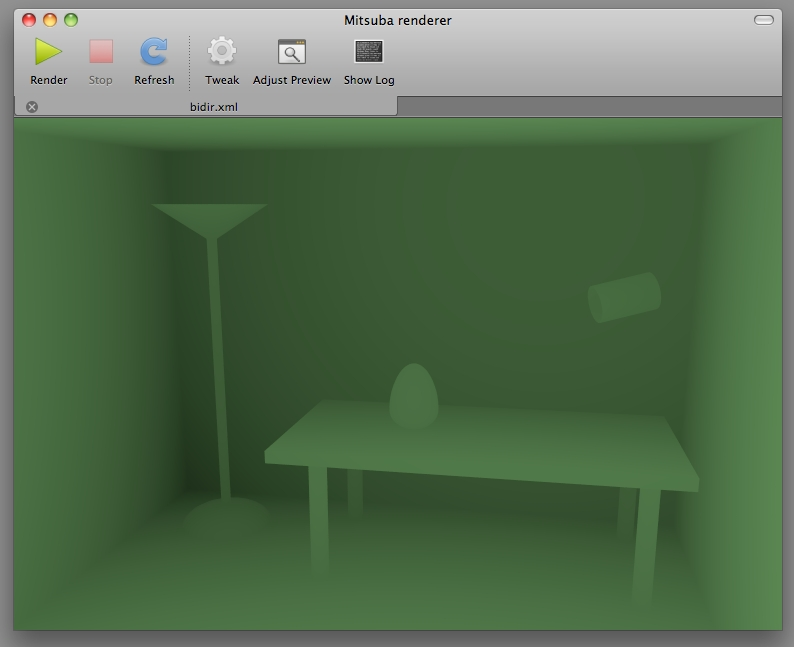
\includegraphics{images/integrator_depth.jpg}}
\end{center}
There are a few more noteworthy details: first of all, the ``usual'' way
to intersect a ray against the scene actually works like this:
\begin{cpp}
	Intersection its;
	Ray ray = ...;
	if (scene->rayIntersect(ray, its)) {
		/* Do something with the intersection stored in 'its' */
	}
\end{cpp}
As you can see, we did something slightly different in the distance
renderer fragment above (we called \code{RadianceQueryRecord::rayIntersect()}
on the supplied parameter \code{rRec}), and the reason for this is \emph{nesting}.
\subsection{Nesting}
The idea of of nesting is that sampling-based rendering techniques can be
embedded within each other for added flexibility: for instance, one
might concoct a  1-bounce indirect rendering technique complete with
irradiance caching and adaptive integration simply by writing the following
into a scene XML file:
\begin{xml}
<!-- Adaptively integrate using the nested technique -->
<integrator type="adaptive">
	<!-- Irradiance caching + final gathering with the nested technique -->
	<integrator type="irrcache">
		<!-- Simple direct illumination technique -->
		<integrator type="direct">
	</integrator>
</integrator>
\end{xml}
To support this kind of complex interaction, some information needs to be passed between the
integrators, and the \code{RadianceQueryRecord} parameter of the function
\code{SamplingIntegrator::Li} is used for this.

This brings us back to the odd way of computing an intersection a moment ago:
the reason why we didn't just do this by calling
\code{scene->rayIntersect()} is that our technique might actually be nested
within a parent technique, which has already computed this intersection.
To avoid wasting resources, the function \code{rRec.rayIntersect} first
determines whether an intersection record has already been provided.
If yes, it does nothing. Otherwise, it takes care of computing one.

The radiance query record also lists the particular \emph{types} of radiance requested
by the parent integrator -- your implementation should respect these as much
as possible. Your overall code might for example be structured like this:

\begin{cpp}
   Spectrum Li(const RayDifferential &r, RadianceQueryRecord &rRec) const {
	  Spectrum result;
      if (rRec.type & RadianceQueryRecord::EEmittedRadiance) {
         // Emitted surface radiance contribution was requested
		 result += ...;
	  }
      if (rRec.type & RadianceQueryRecord::EDirectRadiance) {
         // Direct illumination contribution was requested
		 result += ...;
	  }
	  ...
	  return result;
   }
\end{cpp}
